\documentclass[english]{article}\usepackage[]{graphicx}\usepackage[]{color}
\usepackage{alltt}
\usepackage[T1]{fontenc}
\usepackage[latin9]{inputenc}
\usepackage{geometry}
\geometry{verbose}
\setcounter{secnumdepth}{2}
\setcounter{tocdepth}{2}
\usepackage{amsmath}
\usepackage{graphicx}
\usepackage{esint}
\usepackage{babel}
\usepackage{verbatim} % for \begin{comment}
\usepackage{subcaption}
\IfFileExists{upquote.sty}{\usepackage{upquote}}{}
\begin{document}

\title{Autonomous Robots and Environmental Mapping}

\author{M. Horning, M. Lin, S. Srinivasan, S. Zou}

\maketitle

\begin{abstract}

Compressed sensing is a technique used to reconstruct sparse signals and images while sampling well below the Nyquist rate. Commonly used in fMRIs and medical imaging, we aim to use this technique to allow autonomous robots to map piecewise constant areas of interest within a larger environment. In our experiment, we programmed a robot equipped with a reflectance sensor to travel along straight-line paths on a black testbed with white regions of interest. The robot integrated sensor readings and sent that sum to a remote server after each path. Each data point consists of the robot's start and end positions, tracked by an overhead camera, and the integral found along that path. Once all the data has been collected, the environment is reconstructed by minimizing the sum of the data fitting term and an L1 penalty term. When using an adaptive path selection scheme, preliminary simulations of our experiment show reconstruction of 100x100 images with only 100 data points (relative err. = 0.28), and we have begun trials with data collected by the robot.

\end{abstract}

\pagebreak
\tableofcontents
\pagebreak

\section{Introduction}

\begin{comment}
Discuss Compressed Sensing
\end{comment}

Environment mapping is amongst the foundational problems of mobile robotics. In order for an autonomous vehicle to operate effectively within an environment, 

The task of mapping an unknown environment is well-studied in the area of autonomous robotics. 

Compressed sensing describes a technique in which a signal is reconstructed by solving an underdetermined linear system. Doing so allows a signal to be found from a relatively small amount of data. 

%%%%%%%%%%%%%%%%%%%%%%%%%%%%%%%%%%%% LAB SETUP %%%%%%%%%%%%%%%%%%%%%%%%%%%%%%%%%%%%%%%%%%%%%%%%%%%
\section{Lab Setup}
\subsection{Testbed}
The setup in the UCLA Applied Mathematics Laboratory (AML) used three main components: an overhead camera with a tracking system, a PC computer, and the robot vehicle. The testbed is a 1.5 m x 2.0 m rectangular area made of black asphalt felt paper. The cars' positions are tracked by 2 overhead Imaging Source DMK 21F04 1/4 Monochrome CCD cameras with a resolution of 640 x 480 pixels. They have a frame rate of 30 fps and are connected to an image processing PC via firewire cable. The cars are identified using an OpenCV contour searching function that recognizes black and white ID tags, or "hats", that are fixed on top of the vehicle, giving the robot's current position and orientation \cite{gonzalez2011third}

\subsection{Robot}
\subsection{Video Camera}
\subsection{Server}
\subsection{Putting it all together}
\begin{comment}
Description of testbed, hardware, software, logic
Sid's flowchart
\end{comment}
%%%%%%%%%%%%%%%%%%%%%%%%%%%%%%%%%%%%%%%%%%%%%%%%%%%%%%%%%%%%%%%%%%%%%%%%%%%%%%%%%%%%%%%%%%%%%%%%%%

\section{Models and assumptions}
Our model and lab setup were designed with certain constraints in mind. The model is designed for robots with limited on board storage and computing power. Another limitation is bandwith and infrequent communication with the main server. 

Without loss of generality, we assume the area to be explored is a
rectangle denoted by $\Omega$, and the interested environment variable
$u(x,y)$ is a piece-wise constant function defined on $\Omega$.
See Figure \ref{fig:An-illustration-of-paths} for an illustration.
Assume the robot travels through $n$ different paths, which are denoted
by $C_{1},\ldots,C_{n}$. Along each path $C_{k}$, the integral of
environment variable $u$ is obtained, which is denoted by $g_{k}$.
The path integrals are written as
\begin{equation}
g_{k}=\int_{C_{k}}u(x,y)\mathrm{\,{d}\Gamma},\; k=1,\ldots,n.\label{eq:path-integral}
\end{equation}


\begin{figure}[h]
\begin{centering}

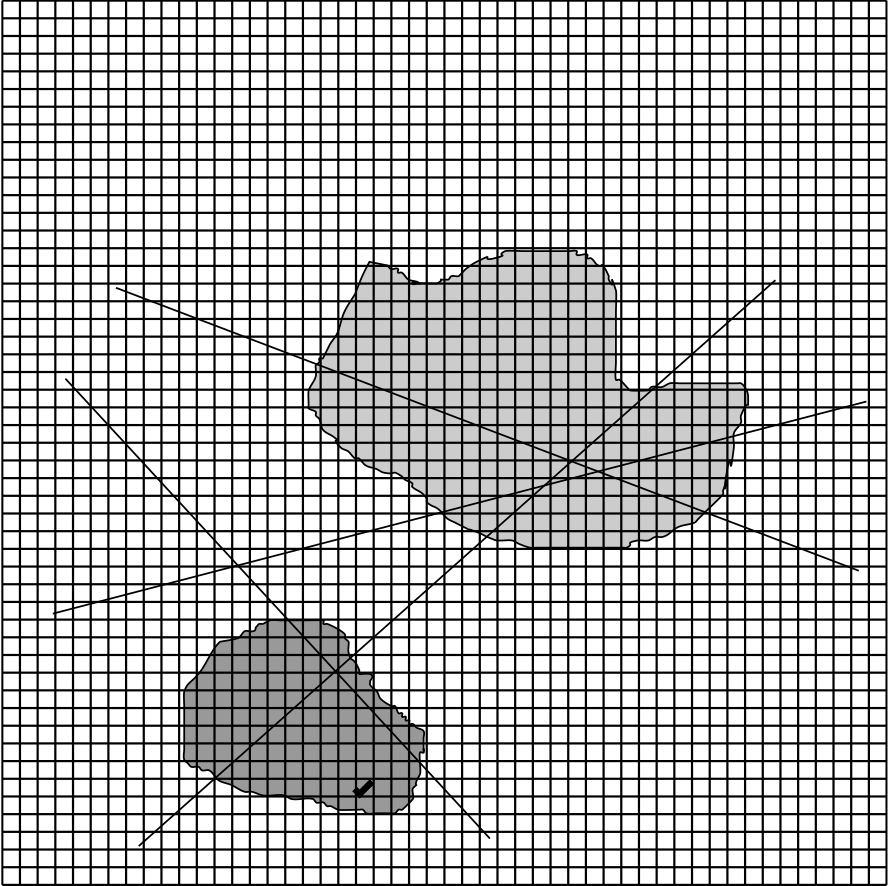
\includegraphics[width=0.5\linewidth]{figures/path-illustration}
\par\end{centering}

\caption{\label{fig:An-illustration-of-paths}An illustration of the paths
of robots. The shaded regions denote the area of interest (unknown),
where the values of environment variable $u$ is significantly different
from the surroundings. The size of the unit pixel (each small rectangle)
is determined by the accuracy of the positioning system.}
\end{figure}


For computational purpose, the whole domain is discretized into rectangular
pixels (See Figure \ref{fig:An-illustration-of-paths}). Each path
$C_{k}$ defines a weight $a_{k,ij}$ for each pixel $(i,j)$. If
$C_{k}$ does not intersect with pixel $(i,j)$, then $a_{k,ij}=0$,
otherwise $a_{k,ij}$ is defined to be proportional to the length
of the part of $C_{k}$ that falls within pixel $(i,j)$. It is also
assumed that the value of $u$ is a constant within each pixel $(i,j)$,
which is denoted by $u_{ij}$. After discretization, Eq (\ref{eq:path-integral})
becomes

\begin{equation}
g_{k}=\sum_{i}\sum_{j}a_{k,ij}u_{ij}.\label{eq:path-integral-discrete}
\end{equation}
Let $g=(g_{1},\ldots,g_{n})^{t}$, $u=(u_{ij})$, then $g$ and $u$
have a linear relation, which is written as 
\begin{equation}
g=Au,\label{eq:system-eq}
\end{equation}
where the linear operator $A$ is specified in Eq (\ref{eq:path-integral-discrete}).
Eq (\ref{eq:system-eq}) is the model equation, which poses an inverse
problem. In this equation, $g$ can be obtained from the experiment,
$A$ is determined by user-specified paths for the robot, which can
be calculated offline. $u$ is the variable that we want to solve.
Of course, if the paths form a complete raster scan over the whole
domain, then theoretically Eq (\ref{eq:system-eq}) has a unique solution.
For economical reasons, it is desirable to use much fewer paths and
still being able to reconstruct a solution for $u$. Inspired by compresed
sensing based image reconstruction techniques, it is hopeful that
reconstruction for our under-determined system can be done.

\begin{comment}
Description of constraints for our problem
limited bandwidth, data storage
Also assumptions about simple piecewise environments
\end{comment}

\section{Algorithm for solving the inverse problem}
\begin{comment}
\end{comment}
\subsection{Simulated Results}
\label{sec:simresults}
\subsection{Experimental Results}

\section{Comparison with Other Approaches}
\begin{comment}
\end{comment}

In order to judge the effectiveness of our approach, we examine other methods of collecting data and reconstructing an image. Perhaps the most intuitive manner in which to gather data about the image is to sample individual points rather than travelling and integrating along a path. As when collecting data in the form of path integrals, we would want the number of sampled points to be as low as possible. Having sampled points for data, there are then multiple approaches to recovering the image. One approach is to simply use the same Split Bregman iteration that we are using for reconstruction from path integrals, but with the individually sampled pixels. Alternatively, we can take the value found at each pixel and assign the same value to nearby pixels, a method that we refer to as pixel expansion.

Figures \ref{fig:samplerec} and \ref{fig:sampleexp} present reconstructions of the previously shown 50x50 test image using these approaches, both with randomly sampled points and points sampled on a grid. In all cases, 100 pixels are sampled, and the sampled points are colored white.

In Figure \ref{fig:samplerec}, Split Bregman iteration was used with the collected data for reconstruction. The algorithm itself is unchanged, but the equation corresponding to a data point will simply give the value of a pixel rather than weighting pixels along the path. This method provides a moderately good reconstruction, especially in determining the general shape of the region of interest in the environment, but the demarcation between the shades of gray in the image is difficult to distinguish, making the image seem very blurry. This is not surprising because by sampling pixels, the only information gathered is about those specific pixels, so the space in between can gradate as quickly or slowly as the reconstruction algorithm deems fit. By comparing Figures \ref{fig:randrec} and \ref{fig:gridrec}, it seems that the reconstruction is more accurate when the points are sampled on a grid. This is reasonable because by sampling on a grid, the spread of sampled points is very even and well distributed. When the points are sampled randomly, certain areas will be less thoroughly investigated than others, hindering accurate reconstruction.

Figure \ref{fig:sampleexp} illustrates pixel expansion. This is done by looping through every pixel in the image, and for each pixel, finding and assigning the value from the nearest pixel that was sampled. This process creates expanded pixels of a single color around each sampled pixel. When the pixels are sampled on a grid, the even distribution causes the expanded pixels to simply be squares, essentially creating a low resolution version of the image, as in Figure \ref{fig:gridexp}. Figure \ref{fig:randexp} is a result of pixel expansion with randomly sampled pixels. The unpredictable spread of sampled pixels causes the expanded pixels to vary widely in shape and size, and the reconstruction does a poor job of determining the shape of the region of interest.

To compare these methods, Figure \ref{fig:othermethoderror} plots the error of these approaches, as well as the path integral reconstruction that we are actually carrying out, with respect to the number of data points collected. The blue line represents reconstruction randomly generated path integrals,

\begin{figure}
\centering
\begin{subfigure}{.5\textwidth}
  \centering
    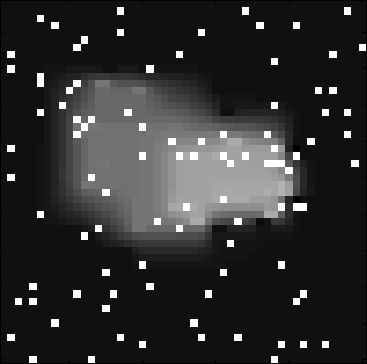
\includegraphics[width=.9\linewidth]{figures/randompointreconstruction}
  \caption{Reconstruction using points sampled randomly.}
  \label{fig:randrec}
\end{subfigure}%
\begin{subfigure}{.5\textwidth}
  \centering
    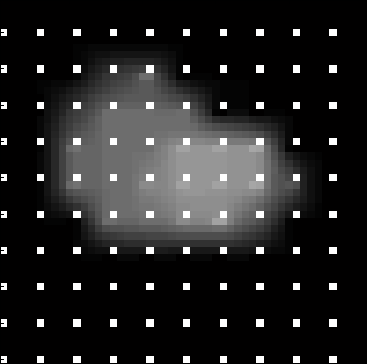
\includegraphics[width=.9\linewidth]{figures/gridpointreconstruction}
  \caption{Reconstruction using points sampled on a grid.}
  \label{fig:gridrec}
\end{subfigure}
\caption{Values are found at sampled points, and Split Bregman iteration is used to reconstruct the image.}
\label{fig:samplerec}
\end{figure}

\begin{figure}
\centering
\begin{subfigure}{.5\textwidth}
  \centering
    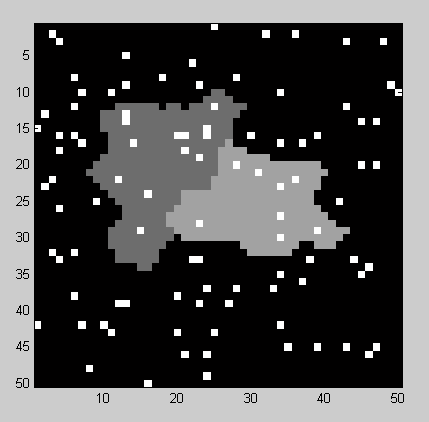
\includegraphics[width=.9\linewidth]{figures/randompointexpansion}
  \caption{Expansion of points sampled randomly.}
  \label{fig:randexp}
\end{subfigure}%
\begin{subfigure}{.5\textwidth}
  \centering
    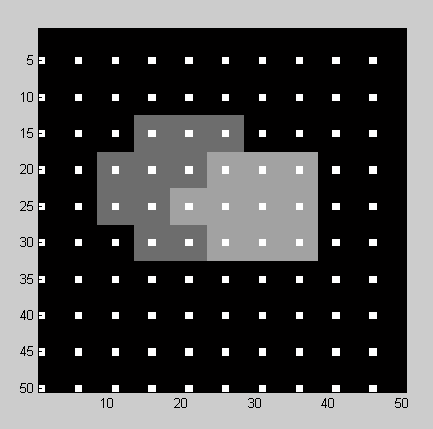
\includegraphics[width=.9\linewidth]{figures/gridpointexpansion}
  \caption{Expansion of points sampled on a grid.}
  \label{fig:gridexp}
\end{subfigure}
\caption{Values are found at sampled points, and those values fill the area surrounding the sampled points.}
\label{fig:sampleexp}
\end{figure}

\begin{figure}
  \centering
    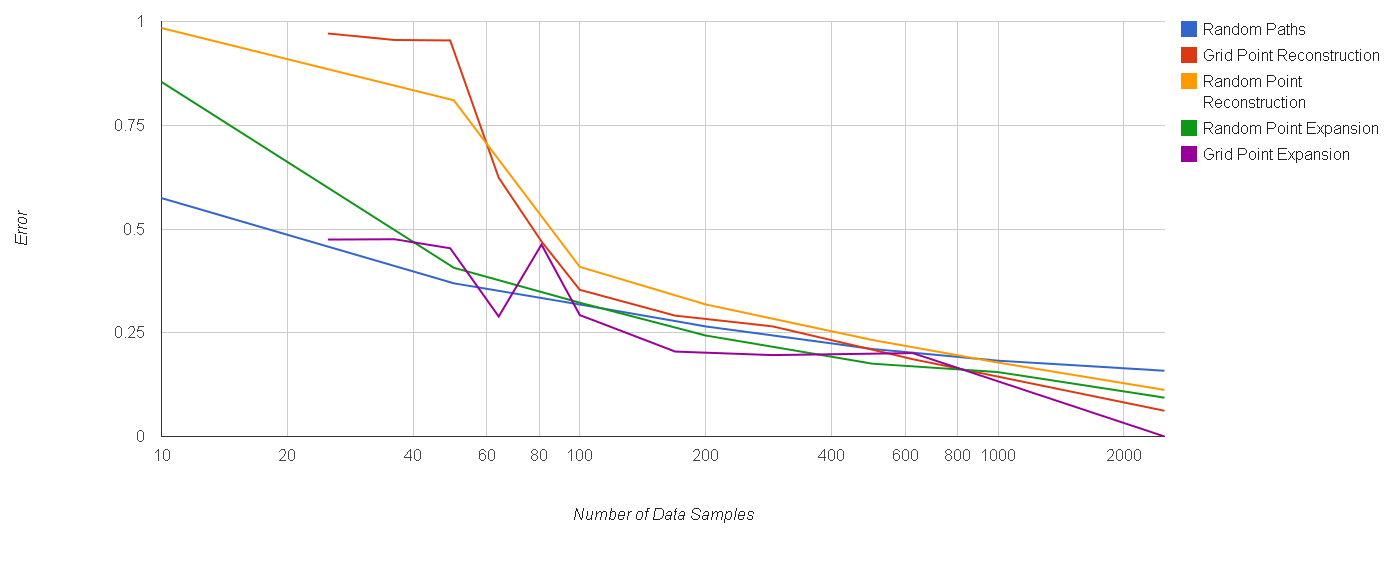
\includegraphics[width=1\textwidth]{figures/othermethoderror}
  \caption{Plot of errors using various reconstruction methods with respect to the number of data samples used.}
  \label{fig:othermethoderror}
\end{figure}

\section{Adaptive Pathing}
\begin{comment}
\end{comment}
\subsection{Simulated Results}
\subsection{Experimental Results}

\section{Conclusions and Further Work}

\newpage
\bibliographystyle{plain}
\bibliography{resources.bib}

\end{document}
